\documentclass[english,14pt]{beamer}
\usetheme{EastLansing}
\usecolortheme{spruce}

\usepackage{xcolor}
\usepackage{listings}
\usepackage{courier}
\usepackage{graphicx}
\usepackage{amsmath}
\usepackage{algorithm2e}
\usepackage{multicol}
\usepackage{hyperref}
\usepackage{textcomp}

% http://mirrors.ibiblio.org/CTAN/macros/latex/contrib/datetime2/datetime2.pdf
\usepackage{babel}
\usepackage[useregional]{datetime2}

% https://tex.stackexchange.com/questions/42619/x-mark-to-match-checkmark
\usepackage{pifont}% http://ctan.org/pkg/pifont

%% https://stackoverflow.com/questions/1435837/how-to-remove-footers-of-latex-beamer-templates
%%gets rid of bottom navigation bars
%\setbeamertemplate{footline}[page number]
%
%gets rid of navigation symbols
\setbeamertemplate{navigation symbols}{}


\usefonttheme[onlymath]{serif}

\definecolor{mGreen}{rgb}{0,0.6,0}
\definecolor{mGray}{rgb}{0.5,0.5,0.5}
\definecolor{mPurple}{rgb}{0.8,0,0.82}
\definecolor{backgroundColour}{rgb}{0.95,0.95,0.92}
\definecolor{lightBlue}{rgb}{0.1, 0.1, 0.8}
\definecolor{darkGreen}{rgb}{0, 0.39, 0}

\newcommand\red[1]{{\color{red} #1}}
\newcommand\green[1]{{\color{green} #1}}
\newcommand\blue[1]{{\color{blue} #1}}
\newcommand\darkGreen[1]{{\color{darkGreen} #1}}

\newcommand{\cmark}{\ding{51}}%
\newcommand{\xmark}{\ding{55}}%

\lstdefinestyle{CStyle}{
    backgroundcolor=\color{backgroundColour},   
    commentstyle=\color{mGreen},
    keywordstyle=\color{magenta},
    numberstyle=\tiny\color{mGray},
    stringstyle=\color{mPurple},
    basicstyle=\footnotesize,
    breakatwhitespace=false,         
    breaklines=true,                 
    captionpos=b,                    
    keepspaces=true,                 
    numbers=left,                    
    numbersep=5pt,                  
    showspaces=false,                
    showstringspaces=false,
    showtabs=false,                  
    tabsize=2,
    language=Python
}

\lstdefinestyle{pseudo}{
        basicstyle=\ttfamily\footnotesize,
        keywordstyle=\color{lightBlue},
        morekeywords={BEGIN,END,IF,ELSE,ENDIF,ELSEIF,PRINT,WHILE,RETURN,ENDWHILE,DO,FOR,TO,IN,ENDFOR,BREAK,INPUT,CONDITIONS},
        morecomment=[l]{//},
        commentstyle=\color{mGreen}
}

\lstset{basicstyle=\footnotesize\ttfamily,breaklines=true}
\lstset{framextopmargin=50pt,tabsize=2}

\title{ENGG1003 - Monday Week 11}
\subtitle{Fitting curves to data: beyond straight-line fit}
\author{Steve Weller}
\institute{University of Newcastle}
%\date{\today}
\date{17 May 2021}

% following is a bit of a hack, but forces page numbers (technically: frame numbers) to run 1,2,3,... 
% with titlepage counting as frame 1

\addtocounter{framenumber}{1}
\titlepage

\begin{document}

\begin{flushleft}
{\scriptsize Last compiled:~\DTMnow}
\vspace*{-5mm}
\end{flushleft}
\framebreak

%==============================================================

\begin{frame}[fragile]

\frametitle{Lecture overview}
\begin{enumerate}
	\item recap: fitting straight line to data
	\item[]
	\item least squares fit
		\begin{itemize}
			\item describe concept of \emph{least squares}
			\item ``do it yourself'' best straight-line fit
			\item Python code to fit a straight line to data (DIY)
		\end{itemize}	
	\item[]
	\item beyond straight-line fit
		\begin{itemize}
			\item Python code to fit a polynomial (eg: parabola, cubic)
		\end{itemize}	
	\item[]
	\item preliminary discussion of the final exam
\end{enumerate}

\end{frame}

%==============================================================

\begin{frame}[fragile]

\frametitle{$1)$ Recap: fitting straight line to data}

\vspace*{-3mm}
\begin{itemize}
	\item recap from Monday week 10, pp.~24--25
	\item output generated by \texttt{linefitdemo.py}
	\item \blue{blue dots: given data} \qquad \red{red line: line-of-best-fit}
\end{itemize}
\vspace*{-3mm}
\begin{figure}[ht]
	\centering
	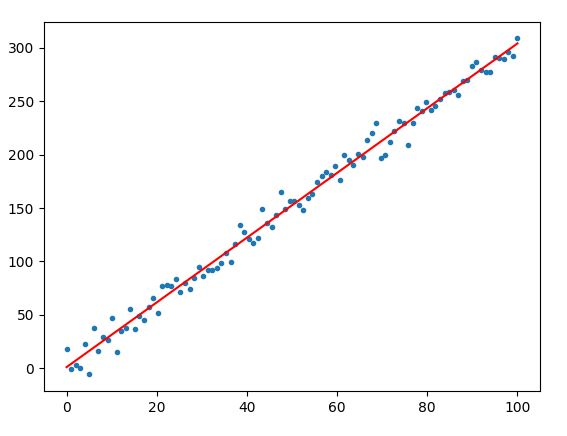
\includegraphics[width=0.68\textwidth]{figures/linefitdemoOutput}
\end{figure}

\end{frame}

%==============================================================

\begin{frame}[fragile]

\frametitle{Recap: line-fitting in Python}

\begin{itemize}
	\item input data consists of $\blue{(x,y)}$ \blue{data pairs}
	\item goal is to calculate gradient $m$ and $y$-intercept $b$ of line-of-best-fit
	\[
		\red{y = mx + b}
	\]
	\item in Python, we use \texttt{curve\_fit()} function in \texttt{scipy.optimize} library to find $m$ and $b$
	\begin{itemize}
		\item may need \texttt{pip install scipy} in terminal
	\end{itemize}
	\item[] \begin{lstlisting}[style=CStyle,basicstyle=\small]
popt, pcov = curve_fit(line, x, y)
m = popt[0]
b = popt[1]
\end{lstlisting}
	\item ignore \texttt{pcov} returned by \texttt{curve\_fit}
\end{itemize}

\end{frame}

%==============================================================

\begin{frame}[fragile]

\frametitle{Two questions}

\begin{enumerate}
	\item how do we define ``best fit''?
	
	\item[]
	
	\item how is equation of line-of-best-fit calculated?
	\begin{itemize}
		\item how does \texttt{curve\_fit()} function in \texttt{scipy.optimize} library actually work?
		\item how are  gradient $m$ and $y$-intercept $b$ actually calculated?
	\end{itemize}

\end{enumerate}

\end{frame}

%==============================================================

\begin{frame}[fragile]

\frametitle{$2)$ Least squares fit}

\begin{itemize}
	\item ``best'' straight-line minimises size of ``error'' between the line and the data points
	\begin{itemize}
		\item definition of ``best'' and ``error'' are somewhat arbitrary\ldots
	\end{itemize}
	\item[]
	\item BUT \red{method of least squares} is standard approach
	\begin{itemize}
		\item overwhelmingly the most commonly used in Engineering
		\item also the basis for more advanced methods
	\end{itemize}

\end{itemize}

\end{frame}

%==============================================================

\begin{frame}[fragile]

\frametitle{Residuals}

% https://kenndanielso.github.io/mlrefined/blog_posts/8_Linear_regression/8_1_Least_squares_regression.html

\vspace*{-3mm}
\begin{figure}[ht]
	\centering
	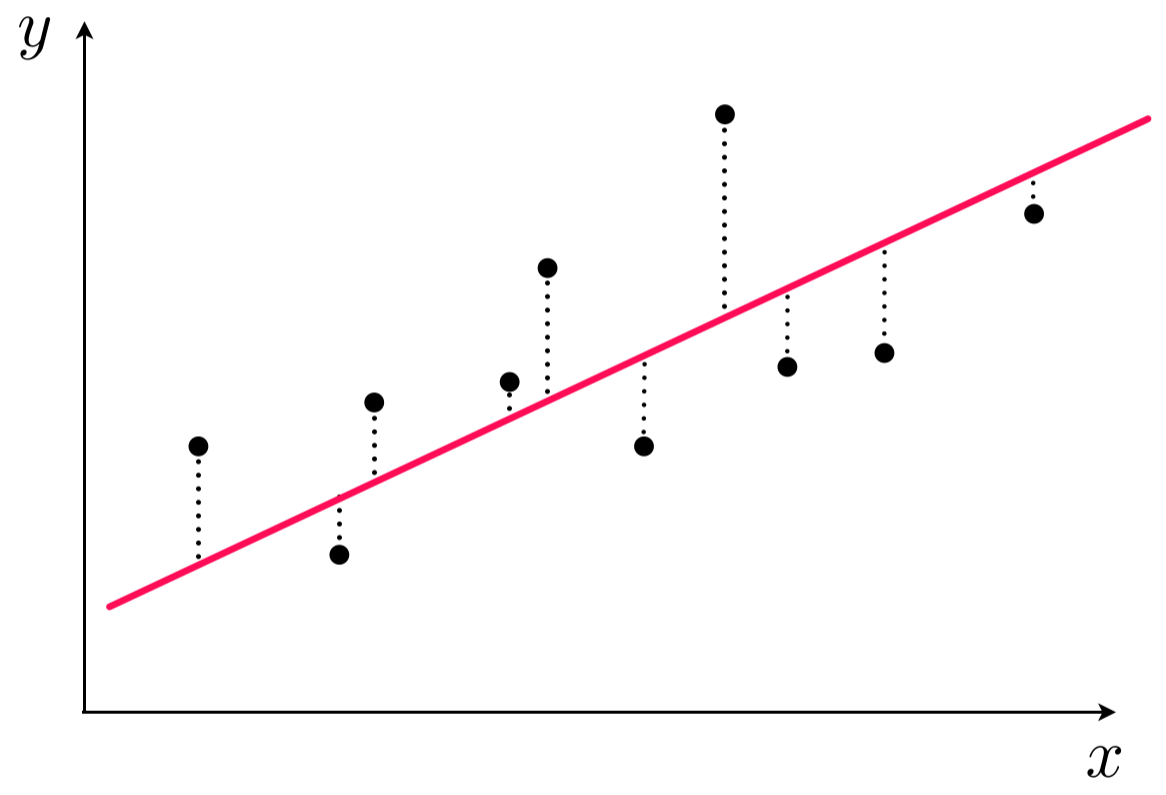
\includegraphics[width=.7\textwidth]{figures/residuals}
\end{figure}
\vspace*{-3mm}
\begin{itemize}
	\item for any choice of straight line, \red{residuals} are shown as dotted lines (different lines $\Rightarrow$ different residuals)
	\item goal is to choose the line with the smallest residuals
\end{itemize}

\end{frame}

%==============================================================

\begin{frame}[fragile]

\frametitle{Method of least squares}

% https://kenndanielso.github.io/mlrefined/blog_posts/8_Linear_regression/8_1_Least_squares_regression.html

\vspace*{-3mm}
\begin{figure}[ht]
	\centering
	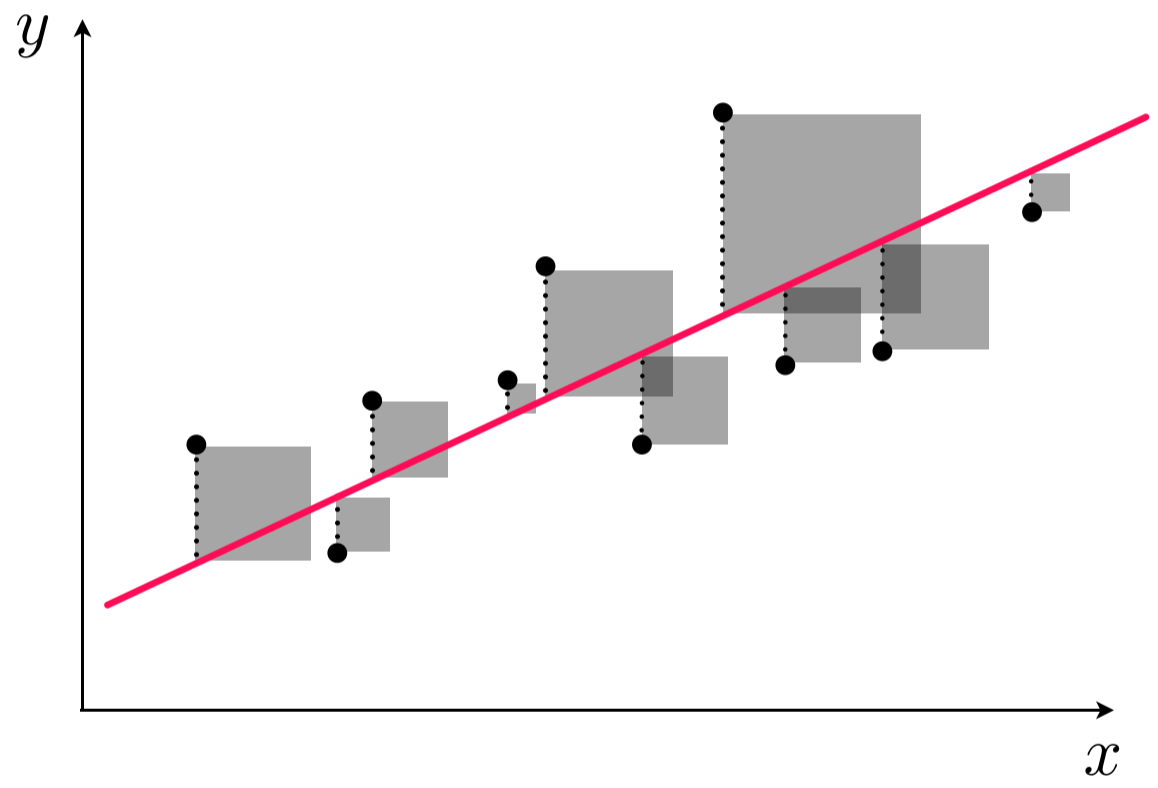
\includegraphics[width=.7\textwidth]{figures/leastsquares}
\end{figure}
\vspace*{-3mm}
\begin{itemize}
	\item method of \red{least squares} calculates the line which makes \emph{total area of grey squares} as small as possible
	\item ie: minimises sum of squares of residuals
\end{itemize}

\end{frame}

%==============================================================

\begin{frame}[fragile]

\frametitle{Method of least squares}

\begin{itemize}
	\item for every choice of $m$ and $b$, can compute total area of grey squares
	\item[]
	\item to find minimum (least value), does that mean we have to search over all possible choices of $m$ and $b$?
	\item[]
	\item \textbf{NO!} --- there are equations for $m$ and $b$ which minimise total area of grey squares
	\item[]
	\item we'll present those equations in a few slides: great opportunity to write some Python code
	\begin{itemize}
		\item compare results with \texttt{curve\_fit()} function in \texttt{scipy.optimize}
	\end{itemize}
\end{itemize}

\end{frame}

%==============================================================

\begin{frame}[fragile]

\frametitle{Sigma notation: $\Sigma$}

\begin{itemize}
	\item equations for best (least squares) choice of $m$ and $b$ use \red{sigma notation}
	\item[]
	\item $\sum$ here denotes ``summing up''
	\[
		\sum_{k=0}^{N-1} x_k = x_0 + x_1 + \cdots + x_{N-1}
	\]
	\item[]
	\item in Python:
	\begin{itemize}
		\item data in length-$N$ array \texttt{x[0], x[1], \ldots, x[N-1]}
		\item use a loop to calculate sum: \texttt{for k in range(0,N)}
	\end{itemize}
\end{itemize}

\end{frame}

%==============================================================

\begin{frame}[fragile]

\frametitle{Least squares straight-line fit}

\begin{itemize}
	\item input data for straight-line fit problem is $N$ pairs
\[
(x_0,y_0), (x_1,y_1), \ldots (x_{N-1},y_{N-1})
\]
\end{itemize}

\textbf{Example:} effect of temperature $T$ on resistance $R$

\begin{center}
 \begin{tabular}{c c} 
$T \;\; (^\mathrm{o}$C) & $R \;$ (ohms) \\
 \hline\hline
20.5 & 765 \\ 

32.7 & 826 \\

51.0 & 873 \\

73.2 & 942 \\

95.7 & 1032 
\end{tabular}
\end{center}

\begin{itemize}
	\item we'll use $x = T$ and $y = R$
\end{itemize}

\end{frame}

%==============================================================

\begin{frame}[fragile]

\frametitle{}

output of \texttt{LSlinefitData.py}
\vspace*{-3mm}
\begin{figure}[ht]
	\centering
	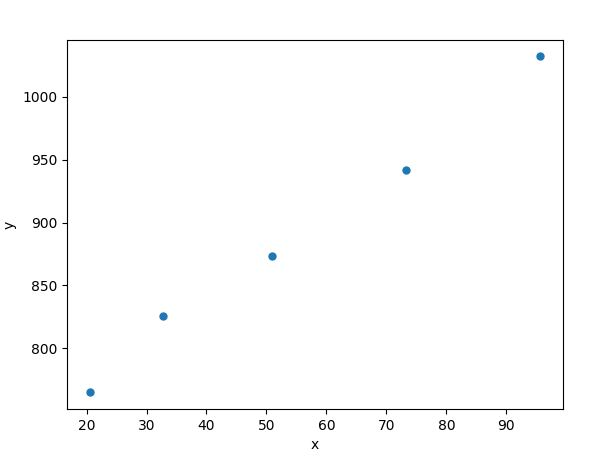
\includegraphics[width=.74\textwidth]{figures/LSlinefitDataOutput}
\end{figure}
\vspace*{-3mm}
{\small \texttt{x = np.array([20.5, 32.7, 51.0, 73.2, 95.7]) } \\
\texttt{y = np.array([765, 826, 873, 942, 1032]) }
}

\end{frame}

%==============================================================

\begin{frame}[fragile]

\frametitle{Least squares straight-line fit}

\textbf{Aim:} find $\mathbf{m}$ and $\mathbf{b}$ in least squares straight-line fit
\[
\boxed{
y = \mathbf{m}x + \mathbf{b}}
\]

\begin{itemize}
	\item define
\[
\red{\bar{\boldsymbol{x}}} = \frac{\sum_{k=0}^{N-1} x_k} {N} \qquad\qquad
\blue{\bar{\boldsymbol{y}}} = \frac{\sum_{k=0}^{N-1} y_k} {N}
\]
	\begin{itemize}
		\item $\bar{x}$ and $\bar{y}$ are averages (means) of $x$ and $y$ arrays
	\end{itemize}
\end{itemize}

\end{frame}

%==============================================================

\begin{frame}[fragile]

\frametitle{Equations for best straight-line fit}
\vspace*{-6mm}
\begin{eqnarray*}
\mathbf{m} & = & \frac{\sum_{k=0}^{N-1}(x_k-\red{\bar{\boldsymbol{x}}})(y_k-\blue{\bar{\boldsymbol{y}}})}{\sum_{k=0}^{N-1} (x_k-\red{\bar{\boldsymbol{x}}})^2} \\[4mm]
\mathbf{b} & = & \blue{\bar{\boldsymbol{y}}} - \mathbf{m} \red{\bar{\boldsymbol{x}}}
\end{eqnarray*}
\vspace*{-7mm}
\begin{lstlisting}[style=CStyle,basicstyle=\footnotesize]
N = len(x)
xbar = np.mean(x)
ybar = np.mean(y)
mnum = 0    # numerator of m
mden = 0    # denominator of m
for k in range(0,N):
    mnum += (x[k]-xbar)*(y[k]-ybar)
    mden += (x[k]-xbar)**2
m = mnum/mden
b = ybar - m*xbar
\end{lstlisting}

\end{frame}

%==============================================================

\begin{frame}[fragile]

\frametitle{}

output of \texttt{LSlinefit.py}
\vspace*{-3mm}
\begin{figure}[ht]
	\centering
	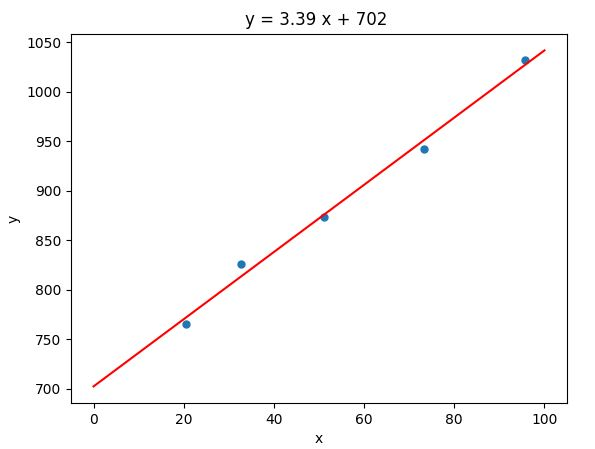
\includegraphics[width=.74\textwidth]{figures/LSlinefitOutput}
\end{figure}
\vspace*{-5mm}
\begin{itemize}
	\item line of best-fit using least squares equations:
	\[
		y = 3.39x + 702
	\]
\end{itemize}

\end{frame}

%==============================================================

\begin{frame}[fragile]

\frametitle{Python code}

\vspace*{-3mm}

\texttt{LSlinefit.py}
\vspace*{-2mm}

\begin{lstlisting}[style=CStyle,basicstyle=\scriptsize]
import numpy as np
import matplotlib.pyplot as plt

def line(x, m, b):
    return m * x + b

x = np.array([20.5, 32.7, 51.0, 73.2, 95.7])    # temp (degC)
y = np.array([765, 826, 873, 942, 1032])  # resistance (ohms)
plt.plot(x, y, '.', markersize=10)
\end{lstlisting}

\begin{itemize}
	\item lines 4--5: prepare to plot straight line obtained by least squares fit
	\item lines 7--9: plot the $(x,y)$ data as blue dots
\end{itemize}

\end{frame}

%==============================================================

\begin{frame}[fragile]

\frametitle{Python code}

\vspace*{-3mm}

\texttt{LSlinefit.py}---continued
\vspace*{-1mm}

\begin{lstlisting}[style=CStyle,basicstyle=\scriptsize]
N = len(x)
xbar = np.mean(x)
ybar = np.mean(y)
mnum = 0    # numerator of m
mden = 0    # denominator of m
for k in range(0,N):
    mnum += (x[k]-xbar)*(y[k]-ybar)
    mden += (x[k]-xbar)**2
m = mnum/mden
b = ybar - m*xbar

xfine = np.linspace(0., 100., 100)
plt.plot(xfine, line(xfine, m, b), 'r')
plt.title('y = {:.2f} x + {:.0f} '.format(m, b))
plt.xlabel('x')
plt.ylabel('y')
plt.show()
\end{lstlisting}

\begin{itemize}
	\item lines 1--10: equations for best straight-line fit
	\item lines 12--13: plot straight-line fit (red line)
\end{itemize}

\end{frame}

%==============================================================

\begin{frame}[fragile]

\frametitle{Straight-line fit using \texttt{curve\_fit()}}

\begin{itemize}
	\item obtain identical results using \texttt{curve\_fit()} function in \texttt{scipy.optimize}
	\item simply replace lines 1--10 on previous slide with:
\end{itemize}

\begin{lstlisting}[style=CStyle,basicstyle=\footnotesize]
popt, pcov = curve_fit(line, x, y)
m = popt[0]
b = popt[1]
\end{lstlisting}

\begin{itemize}
	\item code for \texttt{curve\_fit()} version in \texttt{resistancetemp.py}
	\begin{itemize}
		\item posted in BB and \#lecturecode
	\end{itemize}
\end{itemize}

\end{frame}

%==============================================================

\begin{frame}[fragile]

\frametitle{$3)$ Beyond straight-line fit}

\begin{itemize}
	\item what if data not well described by a straight line?
\end{itemize}
\vspace*{-3mm}
\begin{figure}[ht]
	\centering
	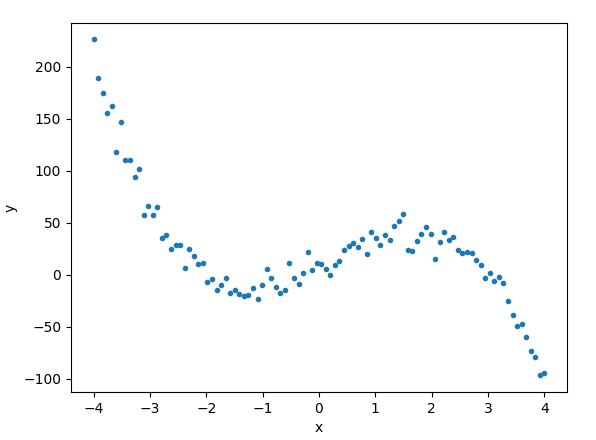
\includegraphics[width=.7\textwidth]{figures/cubicdatapoints}
\end{figure}

\end{frame}

%==============================================================

\begin{frame}[fragile]

\frametitle{Curve-fitting with polynomials}

\begin{itemize}
	\item \texttt{curve\_fit()} function can also be used to fit other curves, eg:
	\begin{itemize}
		\item parabolas: $ax^2 + bx + c$
		\item cubic polynomials: $ax^3 + bx^2 + cx + d$
		\item higher-order polynomials (order-$4$, -$5$ etc)
		\item other ``nonlinear'' functions, eg: $e^{Bx}, \sin(Cx), 1 - e^{-Dx^2}, \ldots$ and combinations of these 
	\end{itemize}
	\item[]	
	\item \texttt{curve\_fit()} uses the method of least squares to fit these curves, too
	\item[]
	\item sometimes physics / creativity / guesswork needed on the ``right'' model to fit
\end{itemize}

\end{frame}

%==============================================================

\begin{frame}[fragile]

\frametitle{Fit parabola to data}
\vspace*{-5mm}
\begin{figure}[ht]
	\centering
	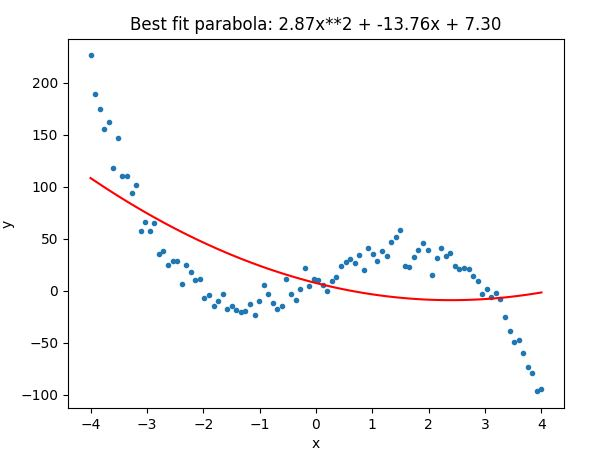
\includegraphics[width=.7\textwidth]{figures/nonlinearguess1output}
\end{figure}
\vspace*{-5mm}
\texttt{curve\_fit()} finds best $a, b, c: \;\; ax^2 + bx + c$

\end{frame}

%==============================================================

\begin{frame}[fragile]

\frametitle{Fit cubic to data}

\vspace*{-5mm}
\begin{figure}[ht]
	\centering
	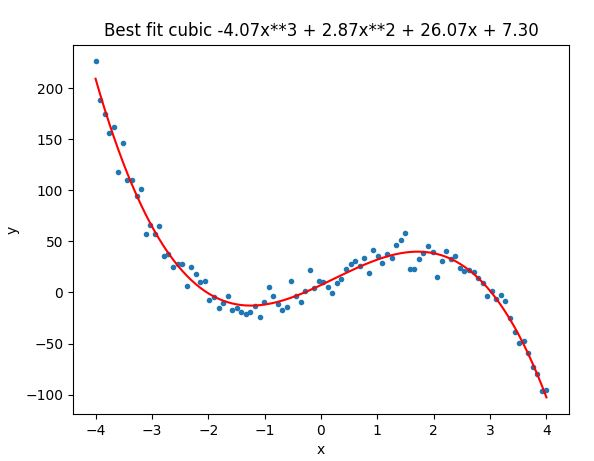
\includegraphics[width=.7\textwidth]{figures/nonlinearguess2output}
\end{figure}
\vspace*{-5mm}
\texttt{curve\_fit()} finds best $a, b, c, d: \; ax^3 + bx^2 + cx + d$

\end{frame}

%==============================================================

\begin{frame}[fragile]

\frametitle{Python code: nonlinearguess1.py}

\vspace*{-3mm}

\begin{lstlisting}[style=CStyle,basicstyle=\scriptsize]
import numpy as np
from scipy.optimize import curve_fit
import matplotlib.pyplot as plt

# guess data is a parabola
def parabola(x, a, b, c):
    return a*x**2 + b*x + c

np.random.seed(1)   # replicate results by fixing seed
# data is actually a cubic + noise
x = np.linspace(-4, 4, 100)
y = -4*x**3 + 3*x**2 + 25*x + 6 + np.random.normal(0., 10, len(x))
plt.plot(x, y, '.')

popt, pcov = curve_fit(parabola, x, y)
a = popt[0]; b = popt[1]; c = popt[2]

plt.plot(x, parabola(x, a, b, c), 'r')
plt.title('Best fit parabola: {:.2f}x**2 + {:.2f}x + {:.2f}'.format(a,b,c))
plt.xlabel('x'); plt.ylabel('y')
plt.show()
\end{lstlisting}

\end{frame}

%==============================================================

\begin{frame}[fragile]

\frametitle{Code commentary}

\begin{itemize}
	\item lines 6--7: fit a parabola to the data: $ax^2 + bx + c$
	\item[]
	\item lines 11--12: data is cubic polynomial $+$ noise
	\begin{itemize}
		\item but \texttt{curve\_fit()} doesn't know this!
	\end{itemize}
	\item[]
	\item lines 15--16 call the \texttt{curve\_fit()} function and ask it to find best-fit parabola
\end{itemize}

\end{frame}

%==============================================================

\begin{frame}[fragile]

\frametitle{Python code: nonlinearguess2.py}

\begin{itemize}
	\item fitting a \emph{cubic} polynomial $ax^3 + bx^2 + cx + d$ to the data requires only a few changes to code in \texttt{nonlinearguess1.py}
	\item see BB for full code listing of \texttt{nonlinearguess2.py}
	\item define cubic function to fit to data:
	\begin{lstlisting}[style=CStyle,basicstyle=\footnotesize]
def cubic(x, a, b, c, d):
    return a*x**3 + b*x**2 + c*x + d
\end{lstlisting}
	\item call \texttt{curve\_fit()} to find best values of $a, b, c, d$
	\begin{lstlisting}[style=CStyle,basicstyle=\footnotesize]
popt, pcov = curve_fit(cubic, x, y)
a = popt[0]; b = popt[1]; c = popt[2]; d = popt[3]
\end{lstlisting}
\end{itemize}

\end{frame}

%==============================================================

\begin{frame}[fragile]

\frametitle{Lecture summary}
\begin{itemize}
	\item least squares fit
	\begin{itemize}
		\item basic concept of least squares
		\item ``do it yourself'' straight-line fit
	\end{itemize}
	\item[]
	
	\item beyond straight-line fit
	\begin{itemize}
		\item fitting polynomials to data
	\end{itemize}
	\item[]
	
	\item preliminary discussion of the final exam
	\item[]
	
\end{itemize}

\end{frame}

\end{document}